\documentclass[a4paper,12pt,fleqn]{article}
\usepackage{fixltx2e}
\usepackage[utf8]{inputenc}
\usepackage{graphicx}
\usepackage{sidecap}
\usepackage{fancyhdr}
\usepackage{amssymb,amsmath}
\usepackage[swedish]{babel}
\usepackage[margin=1.5in]{geometry}
\usepackage{abstract}
\usepackage[parfill]{parskip}
\usepackage{tocloft}
\usepackage{adjustbox}
\usepackage{textcomp}
\usepackage[T1]{fontenc}
\usepackage{pdfpages}
\usepackage{listings}
\usepackage{xcolor,colortbl}
\usepackage{hyperref}

%----------------------------------------------------------------
%C-kod formatering

\definecolor{listinggray}{gray}{0.9}
\definecolor{lbcolor}{rgb}{0.9,0.9,0.9}
\lstset{
backgroundcolor=\color{lbcolor},
    tabsize=4,    
%   rulecolor=,
    language=[GNU]C++,
        basicstyle=\scriptsize,
        upquote=true,
        aboveskip={1.5\baselineskip},
        columns=fixed,
        showstringspaces=false,
        extendedchars=false,
        breaklines=true,
        prebreak = \raisebox{0ex}[0ex][0ex]{\ensuremath{\hookleftarrow}},
        frame=single,
        numbers=left,
        showtabs=false,
        showspaces=false,
        showstringspaces=false,
        identifierstyle=\ttfamily,
        keywordstyle=\color[rgb]{0,0,1},
        commentstyle=\color[rgb]{0.026,0.112,0.095},
        stringstyle=\color[rgb]{0.627,0.126,0.941},
        numberstyle=\color[rgb]{0.205, 0.142, 0.73},
%        \lstdefinestyle{C++}{language=C++,style=numbers}’.
}
\lstset{
    backgroundcolor=\color{lbcolor},
    tabsize=4,
  language=C++,
  captionpos=b,
  tabsize=3,
  frame=lines,
  numbers=left,
  numberstyle=\tiny,
  numbersep=5pt,
  breaklines=true,
  showstringspaces=false,
  basicstyle=\footnotesize,
%  identifierstyle=\color{magenta},
  keywordstyle=\color[rgb]{0,0,1},
  commentstyle=\color{Darkgreen},
  stringstyle=\color{red}
  }
  %-----------------------------------------------------------------
  %marginaler

  \renewcommand{\abstractnamefont}{\normalfont\normalsize\bfseries}
  \renewcommand{\abstracttextfont}{\normalfont\small}
  \renewcommand{\headrulewidth}{0pt}
  \renewcommand{\cftsecleader}{\cftdotfill{\cftdotsep}} 
  \setlength{\absleftindent}{0pt}
  \setlength{\absrightindent}{0pt}
  \setlength{\headheight}{15pt}

  \addtolength{\oddsidemargin}{-.5in}
  	\addtolength{\evensidemargin}{-.5in}
  	\addtolength{\textwidth}{1in}


  %-----------------------------------------------------------------
  %header and footer

  \pagestyle{fancy}
  \lhead{
  	\begin{picture}(0,0)
  		\put(5,0){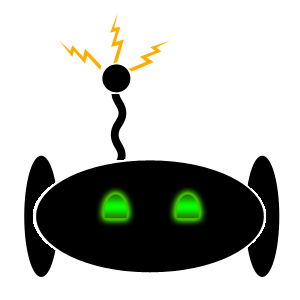
\includegraphics{logotyp.png}}
  	\end{picture}}
	
  \fancyhead[C]{\small{Mapmaster2001}}
  \fancyhead[R]{\small \today}
  \fancyfoot[L]{\small{TSEA56 \\ LIPS Kappa}}
  \fancyfoot[C]{\small{\thepage}}
  \fancyfoot[R]{\small{Projektgrupp 8 \\ mapmaster2001@cyd.liu.se}}

  %-----------------------------------------------------------------

%-------------------------------------------------------------------
%Första sidan
\begin{document}
	\pagestyle{fancy}
\pagenumbering{roman}
	\vspace*{\fill}
		\begingroup
			\begin{center}
				\huge{\textbf{MapMaster 2001}}
				\\
				\vspace{5pt}
				\normalsize
				Kandidatprojekt Y - Grupp 8 - VT2014
				\\
				Version 1.0
				\end{center}
		\endgroup
	\vspace*{\fill}
	
	\begin{center} %Börjar centrering 
		Status
		\\
		\vspace{3pt} %Whitespace 3 pts
	    \begin{tabular}{| p{3cm} | p{3cm} | p{3cm} |} %tabell, 4 horizontella |, 3 cm emellan dem.
	    \hline %översta horizontella linjen.
	    Granskad & - & \today \\ \hline % & -tecken för att "gå till nästa ruta" 
		Godkänd & - & - \\ \hline % avslutas med \\ och \hline.

	    \end{tabular}
	\end{center}
	\vspace{2cm}
	\newpage
%-----------------------------------------------------------------
%Projektidentitet
	
	\vspace*{\fill}
		\begingroup
			\begin{center}
				\LARGE{\textbf{PROJEKTIDENTITET}}
				\\
				\footnotesize
				Grupp 8, 2014/VT, MapMaster2001
				\\
				Linköpings tekniska högskola, ISY
				\\
				\vspace{1cm}
	  \begin{tabular}{| p{3cm} | p{4.3cm} | p{2.4cm} | p{3.8cm} |}
	    \hline
		\textbf{Namn} & \textbf{Ansvar} & \textbf{Telefon} & \textbf{E-post} \\ \hline
	    Jens Edhammer & Dokumentanvsvarig (DOK) & 076-030 67 80 & jened502@student.liu.se \\ \hline
		Erik Ekelund & Designansvarig (DES) & 073-682 43 06 & eriek984@student.liu.se \\ \hline
		David Habrman &  & 976-017 71 15 & davha227@student.liu.se \\ \hline 
		Tobias Grundström & Testansvarig (TES) & 073-830 44 45 & tobgr602@student.liu.se \\ \hline 
		Hans-Filip Elo &   & 073-385 22 32 & hanel742@student.liu.se \\ \hline 
		Niklas Ericson & Projektledare (PL) & 073-052 27 05 & niker917@student.liu.se \\ \hline
	    \end{tabular}
		
		\vspace{1cm}
		\textbf{E-postlista för hela gruppen:} mapmaster2001@cyd.liu.se
		\\[0.5cm]
		
		\textbf{Kund}: Mattias Krysander, Linköpings Universitet, 581 83  LINKÖPING, \\
		013-28 21 98, matkr@isy.liu.se \\
		\textbf{Kontaktperson hos kund}: Mattias Krysander, 013-28 21 98,matkr@isy.liu.se 
		\\
		\textbf{Kursansvarig}: Tomas Svensson, 3B:528,013 28 21 59,tomass@isy.liu.se
		\\[0.5cm]
		\textbf{Handledare}: Peter Johansson, 013-28 1345 peter.a.johansson@liu.se

				\end{center}
		\endgroup
	\vspace*{\fill}
\newpage

%-----------------------------------------------------------------
%Innehållsföreteckning

\addto\captionsswedish{\renewcommand{\contentsname}{Innehållsförteckning}}

\tableofcontents
\thispagestyle{fancy}
\newpage

\pagenumbering{arabic}
%-----------------------------------------------------------------
%Översikt

\section{Inledning}
%''Ge en översiktlig beskrivning av produkten och uppdraget gärna kopplat till bilder.
%Lyft gärna fram det som ni anser är utmanande/intressant i uppdraget. 
%Beskriv kortfattat dispositionen på rapporten.''

En robot med tillgång till ett antal avståndssensorer, en reflexsensor, ett gyro och en RFID-sensor placeras i ett stängt område med dimension på upp till 6x6 meter som är uppdelat i 40x40 centimeters segment. 
Den ska, med en vägg som startpunkt, helt autonomt kartlägga området genom att markera ut var väggar finns och var det finns områden som inte går att nå. 
Den ska även markera ut var det går att finna RFID-taggar, som symboliserar brandhärdar. 
Om inte hela det slutna området är kartlagt ska den upptäcka vilka segment som är oupptäckta, färdas dit och lägga till det i kartan. 
När hela området är kartlagt ska roboten ta sig tillbaka till startpunkten och avsluta arbetet. Ett exempel på en karta kan ses i figur~\ref{fig:omrade}.
\begin{figure}[htp] %Placera här om det finns plats, annars så snart som möjligt, på toppen av en sida.
  \begin{center}
  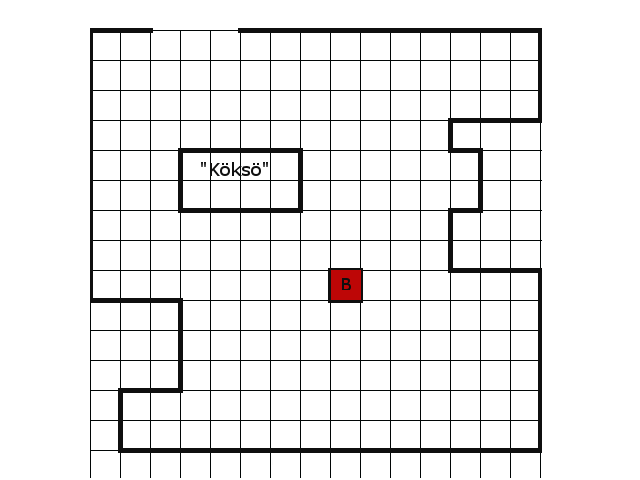
\includegraphics[keepaspectratio=true,scale=0.5]{gimpmap.png}  %skala och filnamn. 
  \end{center}
  \caption{Exempel på område som ska kartläggas} %figurtext.
  \label{fig:omrade}
\end{figure}

Stora delar av arbetet med denna produkt består av att utnyttja den teoretiska kunskap som finns och att koppla den till praktiken för att sedan implementera principerna på roboten. 
Detta innefattar bland annat reglerteori, digitalteknik, sannolikhetslära, optimering och matematisk analys.En av de största utmaningarna med robotens uppdrag är dock att rita ut en karta över området utan att veta var den befinner sig - men hur går det att veta var roboten befinner sig utan en karta?

I denna rapport diskuteras först teori kring att bygga en autonom robot för att sedan gå in på hur vilka metoder vi har använt för att utföra projektet. Därefter ger vi en teknisk beskrivning av de tekniker som vår robot använder sig av samt presenterar resultatet av projektet. Slutligen analyserar vi resultatet och lyfter fram våra reflektioner kring projektet. 

\section{Problemformulering}
%Redogör kort för kravbilden och referera till projektdirektiv och kravspecifikation för %att läsa detaljer.
%Lägg återigen mest fokus på det som ni ansåg utmanande/intressant.

Den slutgiltiga produkten ska uppfylla ett antal krav (Se Kravspecifikation) för att godkännas av beställaren. Principiellt ska roboten kunnas köra autonomt genom ett område (uppbyggt av kartongväggar) och vid rotation skicka en karta till en persondator som på ett prydligt sätt redovisar vad roboten har sett. Roboten ska även kunna detektera brandhärdar som symboliseras med RFID-kort. Dessa kort placeras ut på slumpmässigt valda rutor på banan. 

Kraven som ställts är delvis baserade på vad beställaren ville få levererat (Se Projektdirektiv för kartrobot) och delvis på sådant som projektgruppen ansåg var viktigt för robotens funktionalitet. Ett exempel på funktionalitet som borde prioriteras är hantering av karta och sökalgoritmer, dock så kan det vara så att det även är det svåraste att implementera. Sammanfattningsvis består kraven bland annat av de delar som beskrivs av scenariot i inledningen. Den innehåller även en del krav på vilka delprodukter som ska vara klara vid vissa specifika datum.


\section{Kunskapsbas}

Förutom kunskap från tidigare kurser har litteratur i form av webbsidor och böcker samt personligkontakt med handledare gett stöd och råd. 

\subsection{Personlig kontakt}
Under projektets gång har gruppen haft hjälp av en handledare vid namn Peter Johansson, som är anställd på instutitionen för systemteknik vid Linköpings universitet. 

\subsection{Litteratur}
Den litteratur som använts under projektets gång består till stor del av böcker inom grunderna för bland annat sannolikhetslära, datorteknik\footnote{Roos, Olof. 1995. Grundläggande datorteknik. upplaga 1. Studentlitteratur AB}, elektronik\footnote{Söderkvist, Sune. 1996. Kretsteori och elektronik. utgåva 1. Tryckeriet Erik Larsson AB}, reglerteknik\footnote{Glad, Torkel och Ljung, Lennart (2006), \textit{Reglerteknik - Grundläggande teori}.} och matematisk analys.

\subsection{Webb}
Den ovannämnda litteraturen har kombinerats med datablad för de komponenter som använts tagna från ISY:s sida VanHeden\footnote{\url{https://docs.isy.liu.se/twiki/bin/view/VanHeden}} och datablad från Atmel för de processorer som modulerna baserats på\footnote{\url{http://www.atmel.com/images/doc8059.pdf}}. 
Utöver detta har även diverse forum på internet berörande exempelvis \emph{C}-,\emph{C++}-\footnote{\url{http://stackoverflow.com/}} och \emph{AVR}-programmering\footnote{\url{http://www.avrfreaks.net/}} besökts.


\section{Genomförande}
%Beskriv hur projektet har bedrivits och referera bland annat till LIPS-modellen, %systemskiss, projektplan och designspecifikation. Observera att designspecifikationen %belyser arbetsprocessen och inte den slutliga produkten så om ni uppdaterat %designspecifikationen löpande under projektet så kan ni infoga t ex den version som var %aktuell vid BP3.

Det grundläggande upplägget av projektet har baserats på Lips-modellen\footnote{http://www.liu.se/cul/resurser/lips/kort-beskrivning-av-lips-modellen?l=sv}. Modellen innehåller tre stycken faser. FÖRE, UNDER och EFTER utförandet av projektet. Beslut angående projektets fortskridande har tagits vid så kallade beslutspunkter (förkortas BP) som ligger placerade löpande under de olika faserna. Utöver detta finns det även milstolpar som används för att kunna verifiera att projektet håller tidplanen. 

\subsection{Före}
De dokument som producerades under för-fasen så som systemskiss och projektplan skrevs gemensamt för att alla medlemmar skulle få en så bra inblick som möjligt i hur arbetet planerades. För mer detaljerad beskrivning av arbetsupplägget hänvisas läsaren till ovan nämnda dokument (Se Systemskiss och Projektplan).

\subsection{Under}
Under produktionsfasen började arbetet med att upprätta en designspecifikation. I denna beskrevs robotens struktur som delades upp i 3 stycken moduler. Gruppen delades i 3 och varje delgrupp ansvarade för varsin modul. Modulansvaret hos respektive delgrupp har inneburit förberedande design av delprodukt (Se Designspecifikation) och implementering. 
Vid ett delprojekts slutförande har hårdvaran eller den skrivna koden förklarats för de andra projektmedlemmarna och sedan slagits samman med resten av projektet. 

Dialog hölls även löpande mellan grupperna för att säkerställa att portar och kontakter placerades på smidiga ställen. Vid implementering av mjukvaran har en versionshanteringstjänst vid namn Github använts, detta för att på ett smidigt vis slå samman kod och möjliggöra simultan programmering

Längre in i projektet ändrades grupperna något för att ge alla projektmedlemmar en chans att arbeta med varandra, men även för sprida ut kunskapen kring de olika modulerna.
I slutfasen av projektet turades gruppmedlemmarna om att skriva den tekniska dokumentationen medan andra arbetade med roboten för att effektivisera arbetet.

\subsection{Efter}
I efterfasen överfördes projektresultatet till beställaren och projektet avslutades. En tävling hölls mellan de olika projektgrupperna för att avgöra vilken robot som var bäst. 

\section{Teknisk beskrivning}
%Redovisa det tekniska resultatet och skrivuppgifterna på ett lämpligt sätt. Detaljerade beskrivningar på grindnivå i hårdvaran eller på instruktionsnivå i mjukvaran är i detta sammanhang oftast ointressant. Referera den tekniska dokumentationen och skrivuppgifterna för beskrivning av detaljer. Lyft fram egna kreativa lösningar!
Roboten har implementerats med tre stycken AVR Atmega 1284p-processorer, med en kommunikationsbuss över SPI-länk\footnote{Datablad för Atmega 1284p https://docs.isy.liu.se/twiki/pub/VanHeden/DataSheets/atmega1284p.pdf, hämtad 2014-05-19}. En processor hanterar sensorer, en processor hanterar styrning och en processor agerar kommunikationslänk mellan de två förstnämnda samt en persondatormjukvara över Bluetooth. En processor sitter på det övre kortet och två processorer på det undre kortet, se figur~\ref{fig:robot}

\begin{figure}[htp] %Placera här om det finns plats, annars så snart som möjligt, på toppen av en sida.
  \begin{center}
  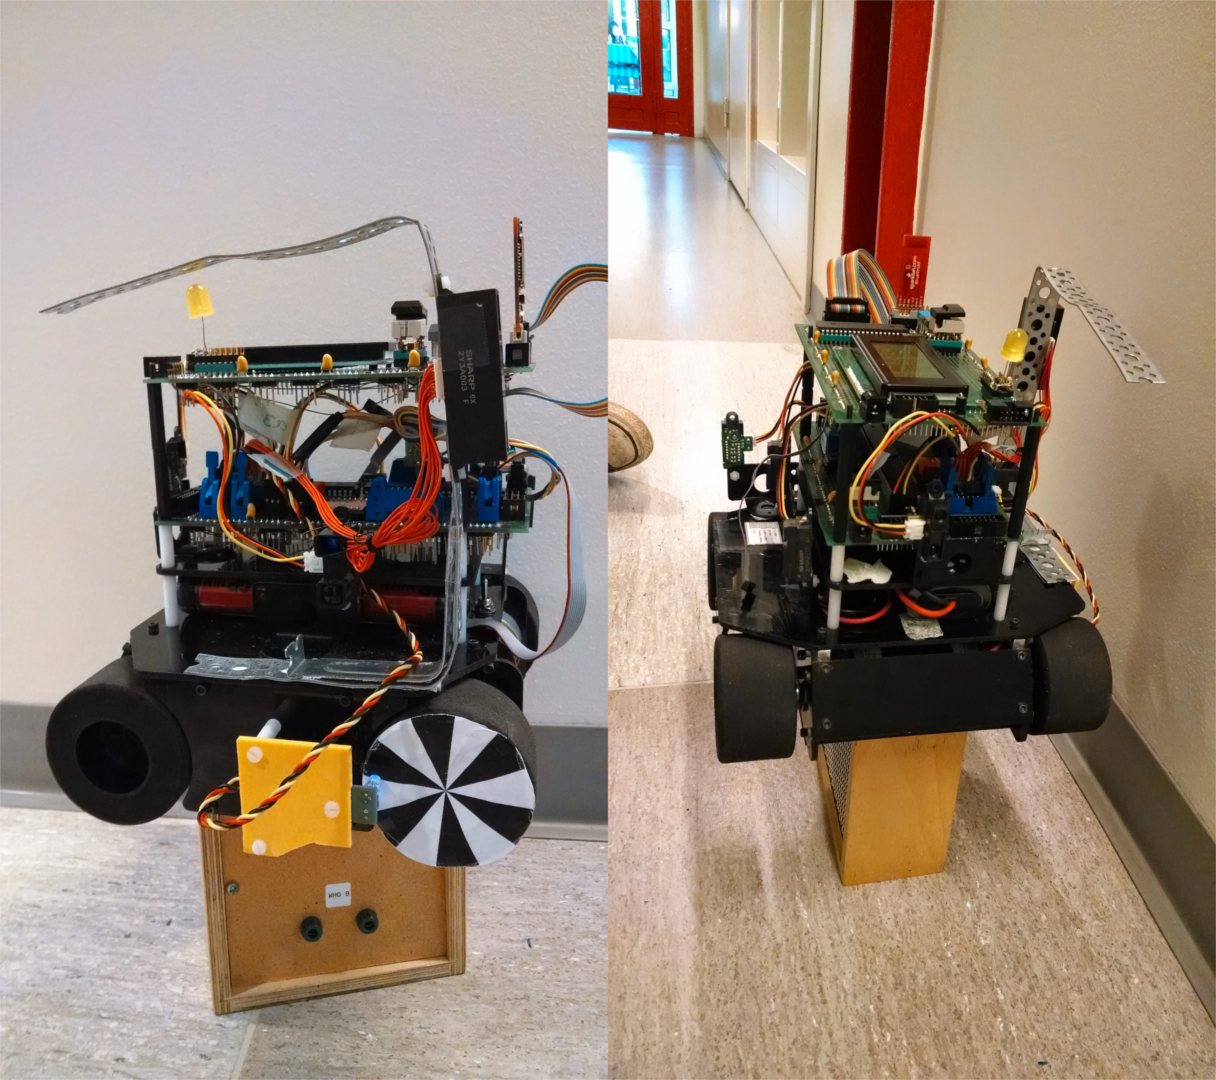
\includegraphics[keepaspectratio=true,width=0.5\textwidth]{robot.png}  %skala och filnamn. 
  \end{center}
  \caption{Bild på roboten från två vinklar} %figurtext.
  \label{fig:robot}
\end{figure}

\subsection{Kommunikation mellan processorer}
Kommunikationen mellan processorerna sker via en Serial Peripheral Interface Bus, hädanefter refererad till som en SPI-buss.
Roboten är konstruerad med tre processorer på två separata vir-kort och kopplas ihop med hjälp av en bandkabel. På roboten agerar kommunikationsmodulen master och de övriga två modulerna är slaves. SPI-bussen kan sammanfattas till att master skiftar ett 8 bitars register med en slave. SPI-bussen har alltså möjlighet för duplex dataöverföring. För ytterligare detaljer angående SPI-bussen se den tekniska dokumentationen.

När master väljer en slave, genom Slave Select signalen, genereras ett avbrott på slave-processorn. Detta innebär att master kan skicka/hämta data i princip var som helst i ett program på en slave-processor. För kommunikation som måste initieras från slave till master har vi kopplat en avbrottssignal som säger till master-processorn att påbörja SPI-kommunikation med aktuell slave-processor.

\subsubsection{Datahantering}
För att avbrotten ska bli så korta som möjligt på processorn så har datahanteringen på kommunikationsmodulen flyttats ut ur avbrott. Anledningen till detta är att så länge processorn befinner sig i avbrott skulle vidare avbrott kunna missas. Sanningsvariabler ifall ny data finns tillgänglig för datahantering används istället. Dessa sanningsvariabler avläses i master-processorns main-loop, vilket visas i flödesdiagrammet i figur~\ref{fig:SPIrec}. Detta ger att nya mottagningar kan påbörjas medan data behandlas, man får dock beakta att data i en given buffer måste behandlas innan den skrivs över av nästa kommunikation.

\begin{figure}[htp] %Placera här om det finns plats, annars så snart som möjligt, på toppen av en sida.
  \begin{center}
  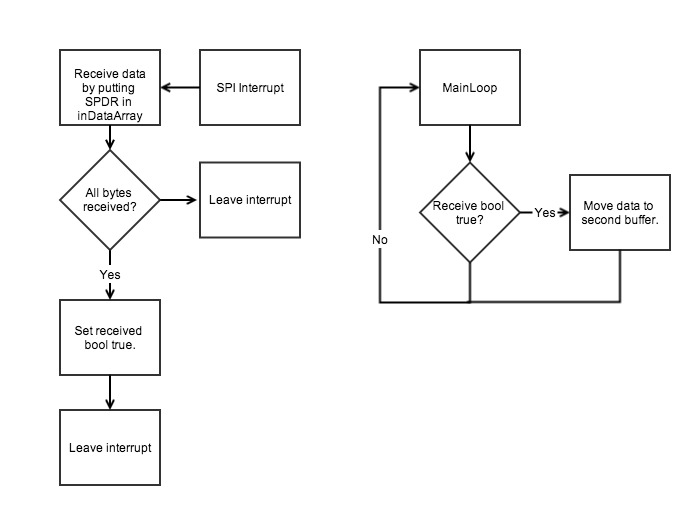
\includegraphics[keepaspectratio=true,scale=0.5]{spirec.jpg}  %skala och filnamn. 
  \end{center}
  \caption{Flödesdiagram för bussmottagning} %figurtext.
  \label{fig:SPIrec}
\end{figure}


\subsubsection{Databufferstruktur}
För att undvika ovannämnda problem utnyttjas en dubbelbuffer. Första buffern är mottagningsbuffern inuti buss-avbrottet. När vi når en databehandlingsfunktion flyttas denna data över till en ny buffer under datahanteringen. Detta innebär att vi kan ta emot ny data från samma sändare på samma buffer sålänge vi har påbörjat databehandling.

\subsection{Kommunikation mellan PC och robot}
Kommunikation mellan processor och PC sker via en Bluetooth-modul. Bluetooth-modulen arbetar via Universal Serial Asynchronous Receiver/Transmitter, USART.
På PC-mjukvaran virtualiseras Bluetooth mottagaren/sändaren som en seriellport och information skickas i form av en 27 element lång char array. För mer detaljer angående dataprotokoll se den tekniska dokumentationen. För en jämförelse mellan olika trådlösa kommunikationstekniker se Appendix~\ref{komuppg.}.

\subsection{PC-mjukvara med grafiskt gränssnitt}

PC-mjukvaran är skapad och designad med hjälp av Open Source varianten av Qt för Mac OS X och dess tillhörande utvecklingsmiljö QtCreator. Qt är ett $C++$ bibliotek som innehåller användarvänliga funktioner för till exempel fönsterhantering och grafisk uppritning.\footnote{\url{http://qt-project.org/}} Ett kompletterande bibliotek till Qt har använts för plottarna kallat QCustomPlot\footnote{\url{http://www.qcustomplot.com/}}.

Med hjälp av mjukvaran kan användaren justera olika parametrar som ändrar robotens beteende vid arbete, till exempel avstånd till väggar som ska hållas, regleringsparametrar och hastighet. Det går att se hur alla sensorers värden ändras över tid, detta kan ses i figur~\ref{fig:gui} och en modell över hur roboten ritar kartan, denna kan även uppdateras genom att användaren trycker på en knapp då autonomt läge ej är aktivt.

Inkluderat i PC-mjukvaran finns ett verktyg för att rita upp tidigare sparade sensorvärden för att lättare kunna analysera hur de förändrats under en körning.

\begin{figure}[htp] %Placera här om det finns plats, annars så snart som möjligt, på toppen av en sida.
  \begin{center}
  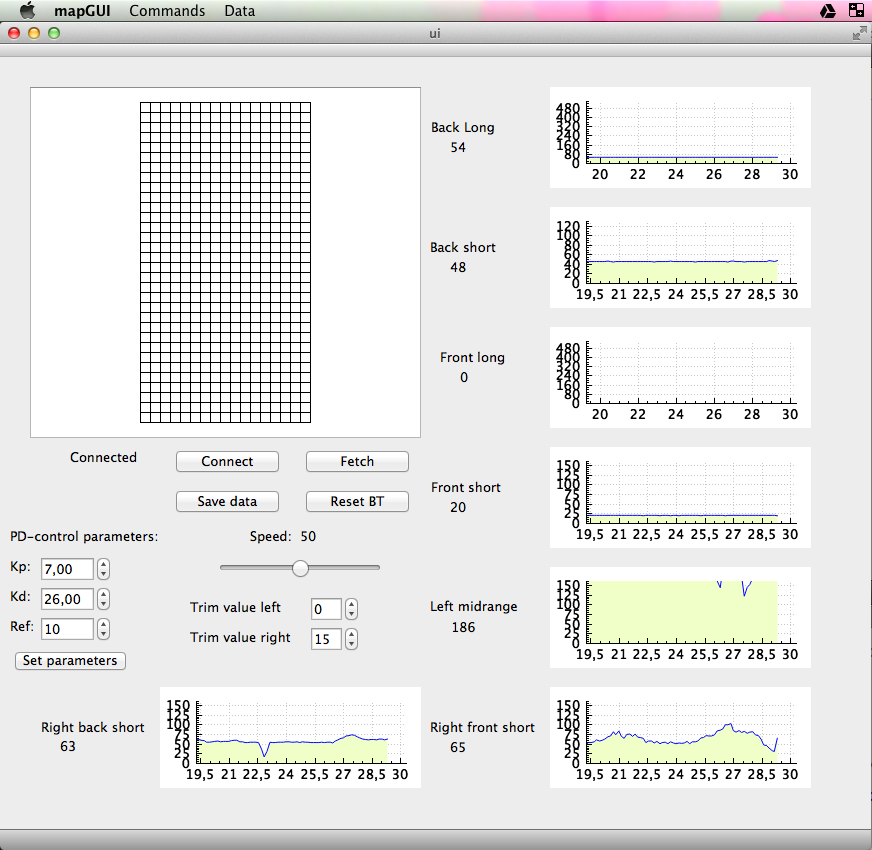
\includegraphics[keepaspectratio=true,width=0.5\linewidth]{gui.png}  %skala och filnamn. 
  \end{center}
  \caption{Det grafiska fönstret} %figurtext.
  \label{fig:gui}
\end{figure}

\subsection{Pulse Width Modulation}

För att styra chassits motorer används AVR-processorns inbyggda pulsbreddsmodulering, PWM. Den som använts är en 8-bitars PWM, det vill säga att den styrs med värden mellan mellan 0 och 255 där 0 innebär att motorerna inte körs och där 255 leder till att roboten kör med 100\% av sin maxhastighet.

PWM fungerar så att en förutbestämd vågform jämförs med en bestämd referensspänning. Utifrån detta genereras en fyrkantsvåg baserat på om den förutbestämda vågen ligger över eller under referenspänningen. När den är över går utsignalen hög och när den är under går utsignalen låg. Detta resulterar i att tiderna som motorn är aktiv respektive avstängd kommer variera beroende på var referensspänningen sätts, vilket leder till olika hastigheter.


\subsection{LCD-display}
LCD-displayen tar relativt processorn lång tid på sig att rita ut ett tecken. Eftersom LCD-displayen hanteras av kommunikationsmodulen, som även är bussmaster, löses displayen utan att processorn väntar på displayen. Detta görs genom att LCD-displayens busyflagga läses i mainloopen och om LCD inte är upptagen skrivs ett tecken ut. För att möjliggöra denna struktur nyttjas en buffer där tecken som ska skrivas ut på displayen hämtas. När alla tecken är skrivna markeras bufferten som klar och vid nästa sensoröverföring skrivs de nya värdena in i bufferten. För detaljer angående LCD-buffern och busyflaggan se den tekniska dokumentationen.

\subsection{Kartabstraktion}


En karta abstraheras i form av en rektangel med ett rutnät med dimensionen 32x17 rutor med koordinaterna (0,0) i det övre vänstra hörnet. Det verkliga området skulle med liknande rutnät bli 16x16 rutor. För att kompensera för eventuella mätfel utökas matrisen något för att underlätta uppritningen. Felaktigheter i avläsning kan leda till att roboten i abstraktionen tillfälligt är utanför sitt givna område. Roboten kommer i början att placeras i punkten (16,1) och rita upp kartan utifrån detta. Det kommer då inte spela någon roll hur roboten är placerad i det verkliga systemet eftersom det finns utrymme för 15 rutor åt båda hållen inklusive marginaler. Koordinatsystemet som används i robotens interna representation är ett vänstersystem, se figur~\ref{fig:coor}

\begin{figure}[htp] %Placera här om det finns plats, annars så snart som möjligt, på toppen av en sida.
  \begin{center}
  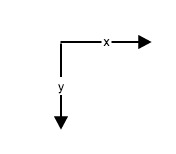
\includegraphics[keepaspectratio=true,width=0.2\textwidth]{coor.jpg}  %skala och filnamn. 
  \end{center}
  \caption{Vänstersystemet som används på roboten} %figurtext.
  \label{fig:coor}
\end{figure}

En abstraktion av en matris i mjukvara skapas med hjälp utav nästlade arrayer, eller någon modern motsvarighet. I utvecklingsmiljön Atmel Studio finns språket C++ tillgängligt, men däremot ej C++ standardbibliotek med abstraktioner.

\subsubsection{Objektklasser}

Kartmatrisen hålls inne i en containerklass med funktioner för att abstrahera access till den. I modern programmering är objekthantering ett kraftfullt verktyg för abstraktion. Klasserna som används följer nedan, med engelska namnet inom parantes.

\begin{itemize}
	\item Karta (Map)
	\item Kartsektion (MapSection)
	\item Robot (Robot)
\end{itemize}

I C++-implementeringen är Robot en dotterklass till MapSection. Detta då alla objekt i en matris måste vara av samma objekttyp. Roboten ärver då vissa egenskaper från MapSection - men innehåller klart mer logik för att hantera positionering och kartläggning. 

MapSection kan anta ett antal olika tillstånd för att markera vilken typ av område det är. Nedan följer de tillstånd som implementerats i klassen MapSection: 

\begin{itemize}
	\item Stängt område (Closed)
	\item Outforskat område (Unexplored)
	\item Tomt område (Empty)
	\item Brandhärd (Fire)
\end{itemize}

Till en början är alla områden outforskade. I takt med att sensordata kommer in och beräknas kan sedan roboten omvandla tillstånden hos objekten i kartan utefter given logik. 

\subsection{Sensormodul}

Roboten har nio olika sensorer. En RFID-läsare, ett gyroskop, en reflexsensor, en långdistansmätare, en mellandistansmätare och fyra kortdistansmätare. 

\subsubsection{AD-omvandling}
De resterande sensorerna ger analoga utsignaler och behandlas med hjälp av en intern A/D-mux på sensormodulen. 
Sensormodulen hämtar kontinuerligt signaler från avståndssensorerna, genom att stega igenom muxen, och från alla sensorer genom att stega igenom muxen. Sensormodulen hoppar, i initialtillståndet, över gyroskopet och reflexsensorn. De analoga insignalerna är lågpassfiltrerade för att ge bättre värden.
För att spara trafik på bussen skapas ett medelvärde av 25 sensorvärden innan de skickas iväg. Samtliga avståndssensorer skickas i gemensam array till kommunikationsmodulen.


\subsubsection{Vinkelhastighetsmätare}
Mätningar på gyroskopet görs på begäran av styrmodulen och låser sensormodulen till enbart gyroskopmätningar. 
Läsningen slutförs när roboten svängt 90 grader och sensormodulen skickar ett kommando till styrmodulen som säger att svängen är klar. Eftersom konstanterna, som modulen använder för att veta när 90 graders rotation är uppnådd, är spänningsberoende finns ett kalibreringskommando för gyrot. Detta kommando utgår från att roboten står still och mäter flera gånger i rad och väljer därefter medelvärdet av mätningarna till nollnivå. Kring nollnivån läggs ett band där värden innanför sägs vara noll grader per sekund, detta för att slippa få mätningar på spänningsrippel. Gyrot nollställs efter att 90 graders svängen är klar och påbörjar inte mätningar igen förän styrmodulen ber om en ny mätning.

\subsubsection{Reflexsensor}
Reflexsensorn, precis som vinkelhastighetsmätaren, körs på begäran av styrmodulen men låser inte sensormodulens avståndsmätningar. Reflexsensorn, som man kan se i figur~\ref{fig:reflex}, tas istället med i muxräkningen. Detta är nödvändigt då vi behöver leverera sensordata under färd tillskillnad från under rotation. Läsningar från reflexsensorn upphör då roboten färdats $40$ cm och sensormodulen skickar ett kommando till styrmodulen
som säger att roboten nått ett nytt segment. Detta kommando skickas upp till tre gånger för att inte missas av kommunikationsmodulen.

\begin{figure}[htp] %Placera här om det finns plats, annars så snart som möjligt, på toppen av en sida.
  \begin{center}
  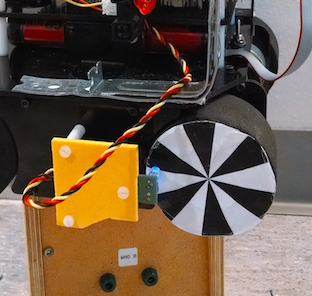
\includegraphics[keepaspectratio=true,width=0.3\textwidth]{reflexsensor.png}  %skala och filnamn. 
  \end{center}
  \caption{Reflexsensor med svartvit-segment på hjulet} %figurtext.
  \label{fig:reflex}
\end{figure}




\subsubsection{RFID-sensor}

RFID-läsaren ger ut en digital signal och behandlas med USART. Vid detektion av en RFID-tagg så stängs USART-avbrott av och ett kommando skickas till styrmodulen som säger till att vi hittat en brandhärd. 
USART-avbrotten stängs av för att inte låsa sensormodulen med flera läsningar av samma tagg. Avbrottet tillåts då roboten lämnat segmentet genom att styrmodulen skickar ett kommando till sensormodulen via kommunikationsmodulen.

\subsection{SLAM}

SLAM står för Simultaneous Localization And Mapping och innebär att roboten ska kunna skatta sin position samtidigt som den ritar upp en karta över området den färdas inom.

\subsubsection{Positionsskattning}
Positionsskattning fungerar genom att reflexsensor uppskattar när roboten rört sig 40 cm. Dessa 40 cm representerar ett segment i vår kartrepresentation och närmre upplösning krävs ej då minsta objektet som ska kartläggas är 40 cm. Roboten innehåller information om vilken riktning den färdas i och får information från sensormodulen om avståndet som färdats. Roboten förflyttas i kartan i aktuell riktning. Vid rotation uppdateras riktningen. 

\subsubsection{Kartläggning}
På styrmodulen ligger en karta i form av en array som uppdateras allteftersom roboten åker och tar in ny mätdata. Arrayen innehåller objekt som kan vara av typen, explored, unexplored, closed och fire. En fördel med att ha objekt i arrayen är t.ex. att funktioner för att överblick och dra slutsatser kring kartan blir väldigt lätta att implementera. T.ex. kan man kolla om en vägg tillhör en köksö genom att helt enkel fråga ett objekt som är closed, isClosed? Ett rekursivt anrop sker då mellan alla närliggande väggar och om väggarna utgör en sluten cirkel, kan hela köksön markes som sluten på kartan. 
Vid sändning av kartan upp till master och sedan vidare till PC-mjukvaran konverteras objekten till bokstäver som sedan avgör färgerna i den uppritande kartan.

\subsection{A-star}
En algoritm vid namn Astar har implementerats för att finna en bra färdväg från punkt A till B i kartan. Algoritmen utgår ifrån Dijkstra's algoritm, som löser problemet att finna billigaste vägen från nod A till B. Den fungerar så att den successivt besöker hörnpunkter i kartan och utgår från startpositionen. Algoritmen expanderar sedan utåt från startpunkten tills målet är hittat. Dijkstra’s algoritm ger garanterat den billigaste vägen, så länge som nodernas kostnader är positiva.\footnote{http://theory.stanford.edu/\textasciitilde amitp/GameProgramming/AStarComparison.html\#the-a-star-algorithm}

Den Giriga Bäst-Först algoritmen fungerar på liknande sätt, förutom att den kan uppskatta hur långt från målet alla hörnpunkter är. Istället för att välja noden som befinner sig närmast startpunkten väljer den här algoritmen den som ligger närmast slutpunkten. Astar algoritmen kombinerar det bästa av dessa två algoritmer och ger alltså garanterat den minst kostsamma vägen, på kortare tid än Dijkstras. \footnote{http://www.policyalmanac.org/games/aStarTutorial.htm}
\newline
I figur~\ref{fig:Astar} visas två exempel på färdväg som Astar-algoritmen har valt vid testning på PC. Färdvägen beskrivs med bokstaven R och vägg/hinder betecknas med bokstaven 0. Startpunkt (S) och slutpunk (F) har slumpats fram. 

\begin{figure}[htp] %Placera här om det finns plats, annars så snart som möjligt, på toppen av en sida.
  \begin{center}
  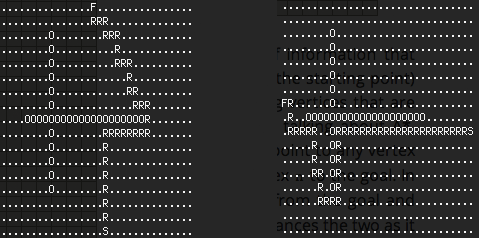
\includegraphics[width=0.75\textwidth]{Astar.png}  %skala och filnamn. 
  \caption{Färdväg efter att Astar-algoritmen har körts på kartan.}%figurtext.
  \end{center}
  \label{fig:Astar}
\end{figure}

\newpage
\section{Resultat}
%Beskriv kortfattat hur produkten används, hänvisa till användarmanualen.

Den slutgiltiga produkten styrs först och främst med hjälp av den tillhörande PC-mjukvaran. Denna mjukvara är utformad för att vara så användarvänlig som möjligt. Det går bland annat att göra små justeringar i robotens beteende utan att behöva skriva om den bakomliggande koden. Användaren kan då enkelt med en Bluetooth-kompatibel dator koppla upp sig mot roboten. Det manuella läget är aktiverat från början och för att styra roboten används endast datorns piltangenter. Roboten stannar då mellanslag trycks. Med ett enda knapptryck kan användaren starta kartläggningen. Detta går även att göra genom att trycka på en knapp på roboten.

När det autonoma läget är aktiverat ska inte användaren behöva göra något utan allt ska sköta sig själv fram till dess att området är kartlagt. En mer detaljerad beskrivning går att finna i användarmanualen för MapMaster2001 (Se Användarmanual)

%Kommentera om produkten klarade de kraven som ställdes upp i kravspecifikationen.

Roboten kan i autonomt läge kartlägga och leta efter RFID-taggar i 25\% av chassits maxhastighet.

De flesta krav med prioritet 1 (se kravspecifikationen) är uppfyllda. Dessa är t.ex. de krav som har att göra med robotens rörelse, de som handlar om kartritning och de flesta krav på autonom körning. Roboten kan följa en högervägg och kartlägga större områden. Den kan dock inte åka genom öppna ytor, de segment som inte gränsar till någon vägg. Således har inte alla krav med prioritet 1 uppfyllts. 

%Beskriv vilken prestanda produkten har och hur det har testats, hänvisa till eventuella %testprotokoll.

Mindre funktioner, så som manuell styrning, kartläggning och avståndssensorernas felmarginal, har testats kontinuerligt under projektets gång. Tester på den slutgiltiga roboten har skett på banor med olika former och storlek. Kartritning, RFID-detektion, positionering, reglering och autonom styrning har då testats.



\section{Slutsatser}
%Slutsatser
Vi är nöjda med projektet i helhet, trots att vi inte uppfyllde alla krav ett. Vi har trots allt gjort en fullt autonom robot som kan navigera och rita upp en karta i 

Det som av projektgruppen ansågs mest utmanande var att konstruera en fullt funktionell buss. Denna ställde till med problem då den i början ofta tappade bitar vilket gav upphov till besynnerligt beteende hos roboten. 

Att få gyrot att fungera var även det en utmaning då det var ytterst viktigt att få rotationerna av roboten så exakta som möjligt. Utan exakta rotationer skulle nämligen roboten kunna positionsuppskatta fel.

Det sista svåra momentet var positionsskattningen. Att simultant positionsskatta och kartlägga visade sig vara lika svårt som förväntat.

%Sammanfatta arbetet. 

%Lyft fram det ni är mest nöjda med.
Vi är väldigt nöjda med är vår implementering av kartritningen, slutning av områden och vår A*-sökalgoritm. Vi är även väldigt nöjda och stolta över objektstrukturen och klass nyttjandet som hela projektgruppen gjort under projektets gång.

%Reflektera över resultatet såväl tekniskt som över genomförandet. Referera efterstudien.ƒ
%Framtida arbete


%Vad skulle ni göra annorlunda om ni skulle göra om samma uppdrag?
Om denna projektgrupp eller någon av dess medlemmar fick göra om detta uppdrag så skulle de använda en multitrådad processor istället för tre. En av de mest tidskrävande aktiviteterna har varit bussen, implementering och felsökning. Bussen är även den del av projektet som gett oss flest fel. Så två saker är säkra, om vi fick möjlighet att göra det utan en buss skulle vi göra det och om vi var tvugna att återigen göra en buss skulle denna påbörjas något tidigare och stresstestas hårt.


%Vad skulle ni vilja utveckla om ni fick mer tid?
Om vi fick mer tid i projektet skulle tiden med all fördel läggas på optimeringsalgoritmer och förbättrandet av bussen. En av förbättringarna till bussen som skulle kunna utnyttjas är en mer avancerad bufferstruktur än den som används.
Roboten har ett delvis färdigt stöd för att förbättra positioneringen med hjälp av avståndssensorerna för att på så sätt kunna ta bort delar av det akumulerande felet som uppstår. Denna funktionalitet fick delvis strykas för att ge tid åt mer essentiella funktioner, då problem uppstod med bussen nära projektets slut. Denna funktion skulle vara intressant att se fullfärdad.  

%Hur skulle ni tänka er att ändra uppgiften för att göra den ännu mer intressant?
I vår åsikt, så skulle tävlingsmomentena kunna göras mer intressanta. I nuvarande form ska RFID-taggar hittas. Dessa taggar måste besökas väldigt långsamt och varje ruta i hela kartan måste besökas för att hitta alla taggar. Detta tar bort väldigt intressanta utmaningar, nämligen avsökningsoptimering, nyttjandet av sensorer med längre räckvidd och en god reglering vid höga hastigheter.

\newpage
\section*{Referenser}
\addcontentsline{toc}{section}{Referenser}

Datablad för Atmega 1284p https://docs.isy.liu.se/twiki/pub/VanHeden/DataSheets/atmega1284p.pdf

http://qt-project.org/

http://stackoverflow.com/

http://www.atmel.com/images/doc8059.pdf

http://www.avrfreaks.net/

http://www.liu.se/cul/resurser/lips/kort-beskrivning-av-lips-modellen?l=sv

http://www.qcustomplot.com/

https://docs.isy.liu.se/twiki/bin/view/VanHeden

Roos, Olof. 1995. Grundläggande datorteknik. upplaga 1. Studentlitteratur AB
Söderkvist, Sune. 1996. Kretsteori och elektronik, utgåva 1. Tryckeriet Erik Larsson AB


% ----------------------------- Appendix -----------------------------------------
% --------------------------------------------------------------------------------

\newpage
\appendix
\pagestyle{empty}
\newgeometry{left=2cm,right=2cm,bottom=2cm,top=2cm}
\section*{Appendix A}
\addcontentsline{toc}{section}{Appendix A}
\label{komuppg.}
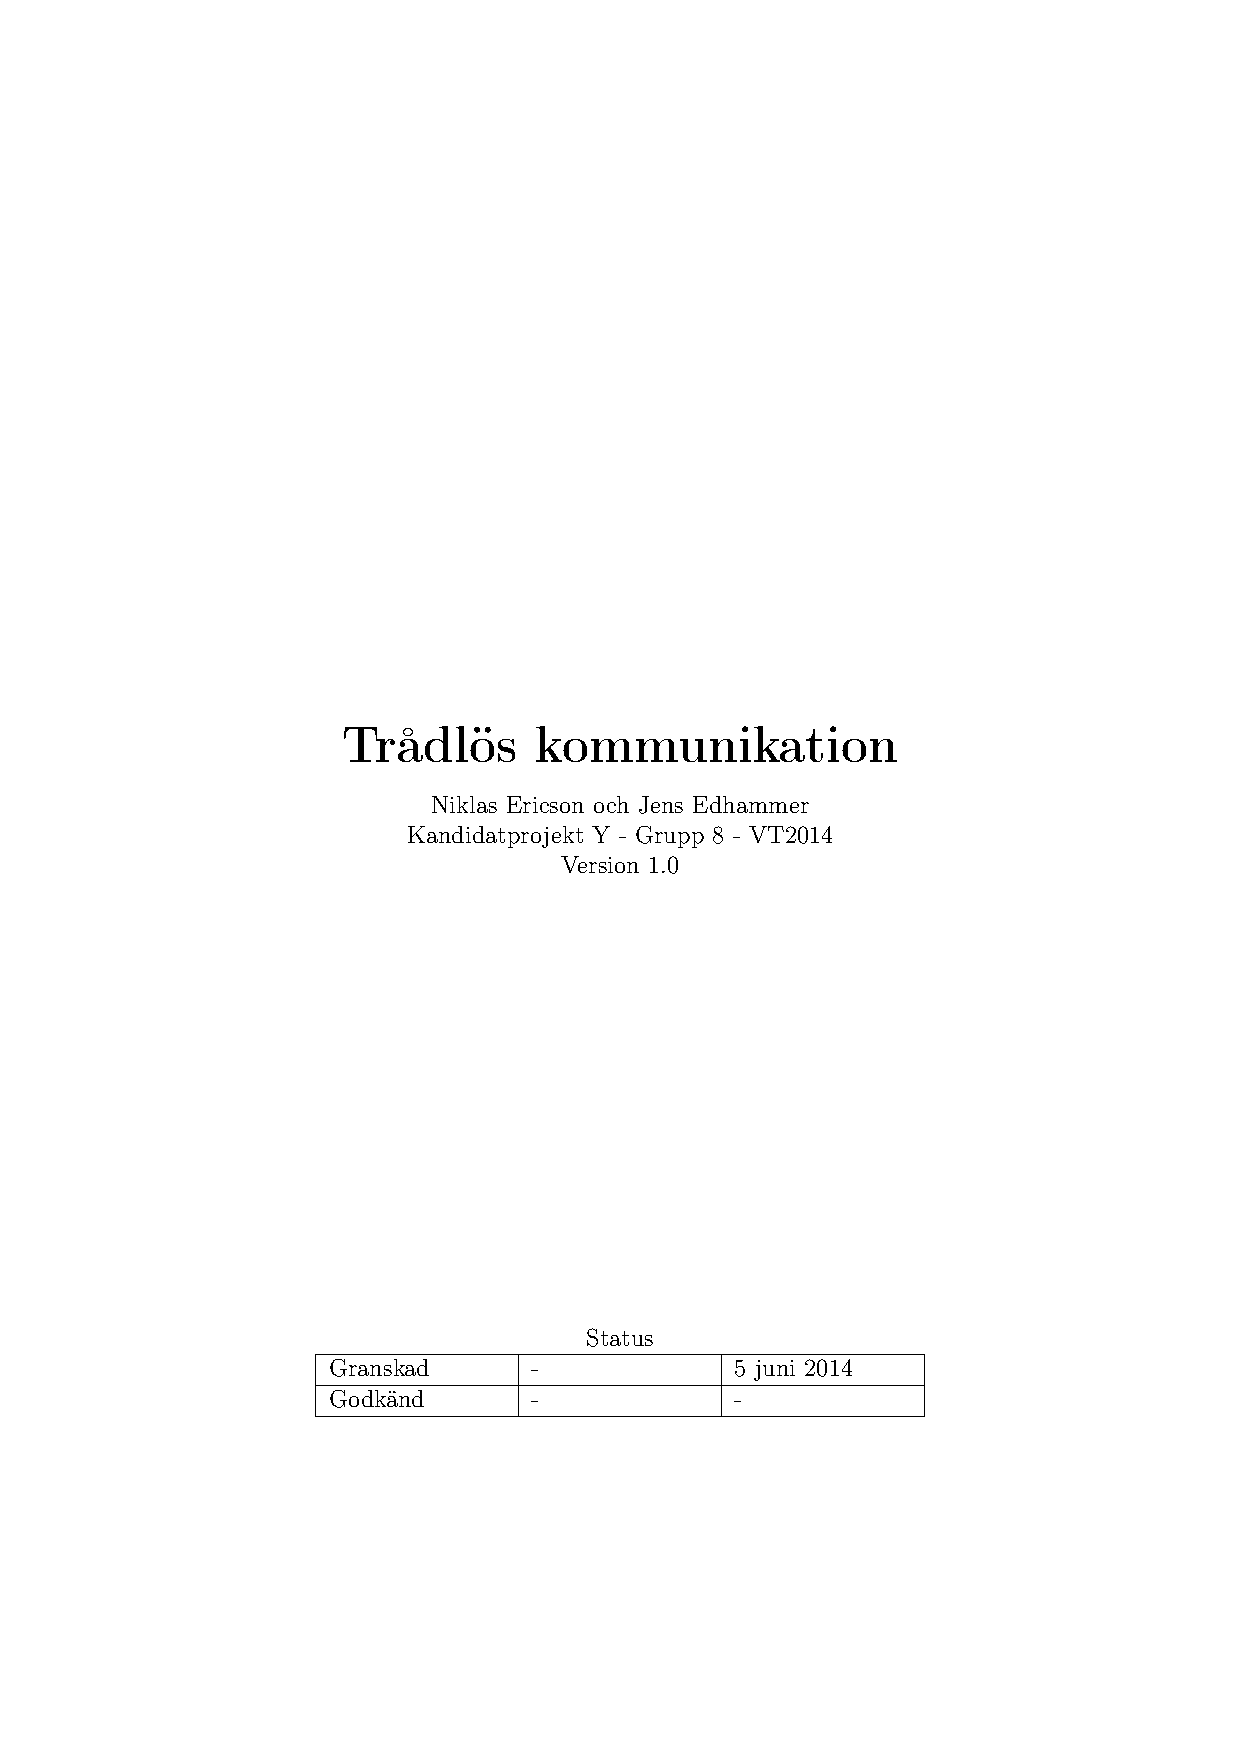
\includepdf[pages=-]{../Kommunikation/kom.pdf}
\section*{Appendix B}
\addcontentsline{toc}{section}{Appendix B}
\includepdf[pages=-]{../Reglering/regler.pdf}
\section*{Appendix C}
\addcontentsline{toc}{section}{Appendix C}
\includepdf[pages=-]{../Sensorer/Sensorer.pdf}

%\section{Appendix B}
%\includepdf[pages=-]{../Regler/regler.pdf}

%\section{Appendix C}
%\includepdf[pages=-]{../Sensorer/Sensor.pdf}


%LIPS-dokument och fördjupningar enligt ovan.
\end{document}
